%%%%%%%%%%%%%%%%%%%%%%%%%%%%%%%%%%%%%%%%%%%%%%%%%%%%%%%%%%%%%%%%%%%%%%%%%%%%%%%%%%%%%%%%%%%%%%%%%%%%%%%%%%%%%%%%%%%%%%%%%%%%%%%%%%%%%%%%%%%%%%%%%%%%%%
% 20141006 - Introduction to Operating Systems VO
%%%%%%%%%%%%%%%%%%%%%%%%%%%%%%%%%%%%%%%%%%%%%%%%%%%%%%%%%%%%%%%%%%%%%%%%%%%%%%%%%%%%%%%%%%%%%%%%%%%%%%%%%%%%%%%%%%%%%%%%%%%%%%%%%%%%%%%%%%%%%%%%%%%%%%

\tikzstyle{block} = [rectangle, draw, fill=blue!20, 
    text width=10em, text centered, rounded corners, minimum height=3em]
\tikzstyle{info} = [rectangle, draw, 
    text width=10em, text centered, rounded corners, minimum height=3em]

%fancyhdr
\lhead{IOS VO} 
\rhead{2014-10-06}

%%%%%%%%%%%%%%%%%%%%%%%%%%%%%%%%%%%%%%%%%%%%%%%%%%%%%%%%%%%%%%%%%%%%%%%%%%%%%%%%%%%%%%%%%%%%%%%%%%%%%%%%%%%%%%%%%%%%%%%%%%%%%%%%%%%%%%%%%%%%%%%%%%%%%%

\par{
    \noindent
    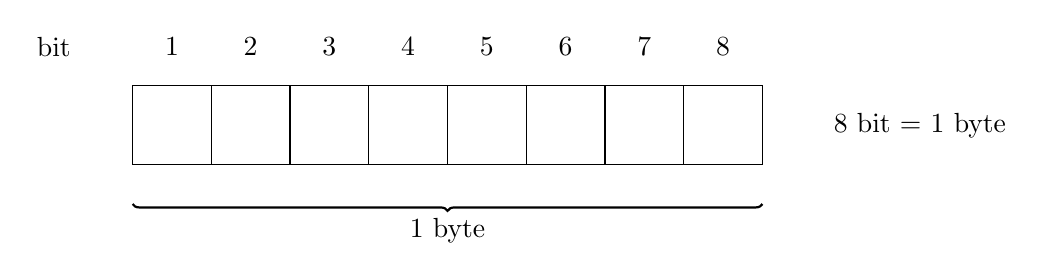
\begin{tikzpicture} 
        \draw (1, 0) rectangle (9, 1);
        \foreach \x in {1, 2, 3, 4, 5, 6, 7} {
            \draw (\x + 1, 0) -- (\x + 1, 1);
            \node at (\x + 1 - 0.5, 1.5) {\x};
        }
        \node at (8.5, 1.5) {8};
        \node at (0, 1.5) {bit};
        \node at (11, 0.5) {8 bit = 1 byte};

        \draw [thick, decoration={ brace, mirror, raise=0.5cm}, decorate]
            (1, 0) -- (9, 0)
            node [pos=0.5,anchor=north,yshift=-0.55cm] {1 byte};
    \end{tikzpicture}
}

\par{
    \noindent
    \underline{Byte-addressing and word-alignment:}
    \par{
        \noindent
        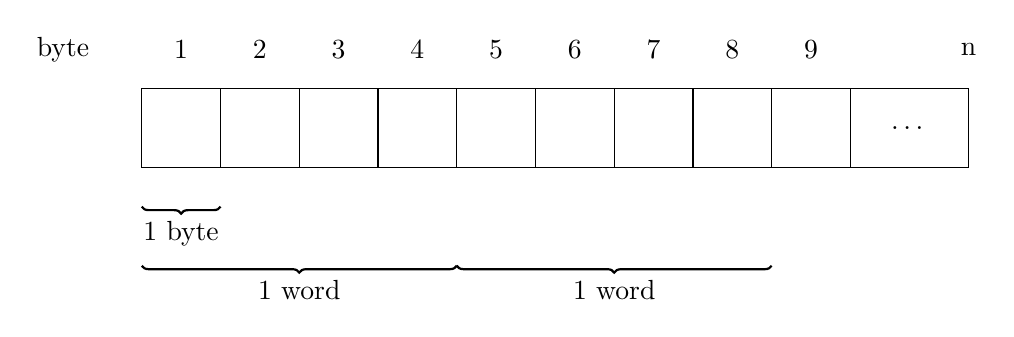
\begin{tikzpicture}
            \draw (1, 0) rectangle (11.5, 1);
            \foreach \x in {1, 2, 3, 4, 5, 6, 7, 8, 9} {
                \draw (\x + 1, 0) -- (\x + 1, 1);
                \node at (\x + 1 - 0.5, 1.5) {\x};
            }
            \node at (10.75, 0.5) {\ldots};
            \node at (11.5, 1.5) {n};
            \node at (0, 1.5) {byte};

            \draw [thick, decoration={ brace, mirror, raise=0.5cm}, decorate]
                (1, 0) -- (2, 0)
                node [pos=0.5,anchor=north,yshift=-0.55cm] {1 byte};
            \draw [thick, decoration={ brace, mirror, raise=0.5cm}, decorate]
                (1, -0.75) -- (5, -0.75)
                node [pos=0.5,anchor=north,yshift=-0.55cm] {1 word};
            \draw [thick, decoration={ brace, mirror, raise=0.5cm}, decorate]
                (5, -0.75) -- (9, -0.75)
                node [pos=0.5,anchor=north,yshift=-0.55cm] {1 word};
        \end{tikzpicture}
    }
}

\par{
    \noindent
    Wie funktioniert der Zugriff auf den Stack? \newline
    Wieso wird \texttt{R1, R28, -4} gemacht? \textbf{Latency}.
}

\par{
    \noindent
    \underline{Implementation von \texttt{void* malloc(int s)}:}
    \par{
        \indent\texttt{LDW 1, 29, 12} \newline
        \indent\texttt{ADD 27, 0, 26} \newline
        \indent\texttt{ADD 26, 26, 1} \newline
    }
    \par{
        \noindent
        \texttt{s}: \texttt{R1 = sum[R29 + 12]} \newline
        Da man in \texttt{C$^*$} keinen Zugriff auf Register hat, muss obiges Verhalten per Assembler implementiert werden. \newline
        \texttt{malloc} ist in der (g)libc enthalten und ist heutzutage de facto ein Betriebssystemfeature.
    }
    \par{
    	\noindent\underline{Implementation von \texttt{int getchar()}:} \newline
        \indent\texttt{RDC 0, 0, 27}
    }
    \par{
    	\noindent\underline{Implementation von \texttt{void putchar(int c)}:} \newline
        \indent\texttt{LDW 1, 29, 12} \newline
        \indent\texttt{WRC 0, 0, 1}
    }
    \par{
    	\noindent
    	Liest den n{\"a}chsten Character aus einem Stream. \newline
    	\texttt{R27 = getchar();} \newline
    	Streams: \texttt{stdin}, \texttt{stdout}, \texttt{stderr}
    }
    \par{
        \noindent
        \begin{figure}[H]
            \centering
            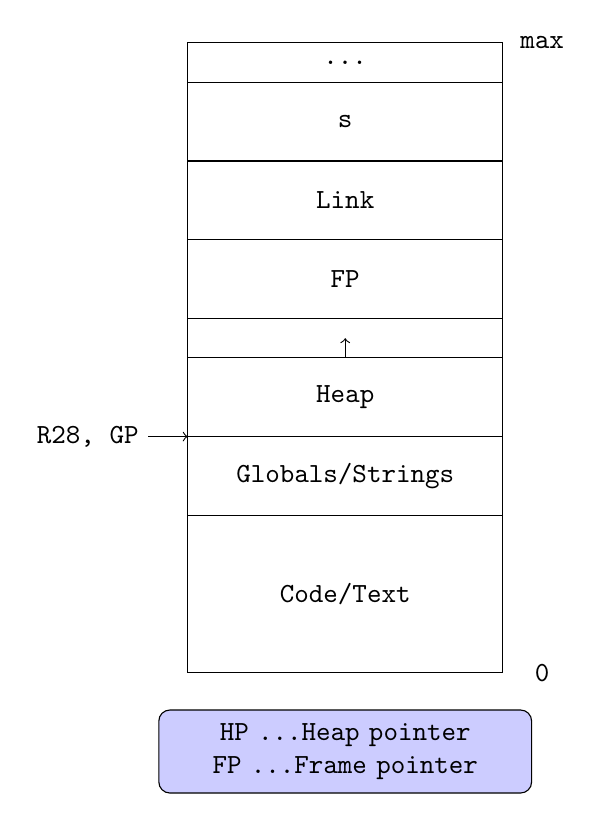
\begin{tikzpicture}
                \draw (2, 1.5) rectangle (6, 9.5);
                
                \node at (6.5, 1.5) {\texttt{0}};
                \node at (6.5, 9.5) {\texttt{max}};

                \draw (2, 9) -- (6, 9);
                \node at (4, 9.25) {\texttt{\ldots}};
                
                \draw (2, 8) -- (6, 8);
                \node at (4, 8.5) {\texttt{s}};

                \draw (2, 7) -- (6, 7);
                \node at (4, 7.5) {\texttt{Link}};

                \draw (2, 6) -- (6, 6);
                \node at (4, 6.5) {\texttt{FP}};

                \draw (2, 3.5) -- (6, 3.5);
                \node at (4, 2.5) {\texttt{Code/Text}};
                
                \draw (2, 4.5) -- (6, 4.5);
                \node at (4, 4) {\texttt{Globals/Strings}};

                \draw (2, 5.5) -- (6, 5.5);
                \node at (4, 5) {\texttt{Heap}};
                \draw[->] (4, 5.5) -- (4, 5.75);
                \draw[<-] (2, 4.5) -- (1.5, 4.5) node[left]{\texttt{R28, GP}};

                \node[block] at (4, 0.5) [text width = 4.5cm]{\texttt{HP \ldots Heap pointer FP \ldots Frame pointer}};
            \end{tikzpicture}
            \caption{Memory layout revisited}
            \label{fig:memorylayout}
    	\end{figure}
    }
    \par{
	    \noindent
	    \textbf{F2}
	}
	\par{
	    \noindent
	    \begin{tabular}{llll}
	        \hline
	        Instruction 	& Semantics 						& Additional information	\\
	        \hline
	        \hline
	        \texttt{RDC c}  &   \texttt{reg[c] = getchar();}	& 							\\
	                        &   \texttt{pc:=pc+4;}				&              				\\
	        \texttt{WRC c}  &   \texttt{putchar(reg[c]);}		& 							\\
	                        &   \texttt{pc:=pc+4;}				& 							\\
	        \hline
	    \end{tabular}   
	}
	\par{
		\noindent
		Why is it so hard to implement \texttt{RDC} and \texttt{WRC} on application level? Because operating systems stuff is self-referential!
		\begin{figure}[H]
			\centering
			\begin{tikzpicture}
				\node[draw, minimum width = 4cm, minimum height = 2cm] (processor) at (0, 0) {processor};
				\node[draw, minimum width = 4cm, minimum height = 2cm, above = -0.015 of processor] (appC) {application in \texttt{C$^*$}};

				\node[right = 0 of processor.north east, text width = 0.5em] (os_t) {OS, DLX};
			\end{tikzpicture}
			\caption{Application and processor}
            \label{fig:appandproc}
		\end{figure}
	}
	\par{
		\noindent
		How does I/O work on a processor?
		\begin{figure}[H]
			\centering
			\begin{tikzpicture}
				\node[draw, minimum width = 3cm, minimum height = 3cm] (processor) at (0, 0) {};
				\node[draw, right = 0.125 of processor.west] (cpu) {CPU};
				\node[draw, above left = 0.25 and 0.125 of processor.east] (in1) {};
				\node[draw, below left = 0.25 and 0.125 of processor.east] (in2) {};
				\node[above = 0.125 of processor.north east] (data_t) {data};
				\node[below = 0.125 of processor.south east] (control_t) {control};
				\draw[dashed] (data_t.south) -- (in1.north);
				\draw[dashed] (control_t.north) -- (in2.south);

				\node[draw, right = 1 of processor, minimum width = 1.75cm, minimum height = 1.2cm] (rs232) {};
				\node[draw, below right = 0.125 and 0.125 of rs232.north west] (rs232_1) {\tiny{1}};
				\node[draw, right = 0.125 of rs232_1] (rs232_2) {\tiny{2}};
				\node[draw, right = 0.125 of rs232_2] (rs232_3) {\tiny{3}};
				\node[draw, below = 0.125 of rs232_1] (rs232_4) {\tiny{4}};
				\node[draw, right = 0.125 of rs232_4] (rs232_5) {\tiny{5}};
				\node[draw, right = 0.125 of rs232_5] (rs232_6) {\tiny{6}};
				\node[below = 0 of rs232.south] (rs232_t) {RS232};
				\node[right = 0 of rs232.east] (ascii_t) {ASCII};

				\draw[<->, >=stealth, thick] (processor.east) -- (rs232.west);
			\end{tikzpicture}
			\caption{I/O on a processor}
            \label{fig:ioproc}
		\end{figure}
	}
}

\par{
	\noindent\underline{Computability \& Complexity of algorithms}
	\par{
		\noindent
		What is the minimal machine that is still universal?
		\begin{itemize}
			\item{
				RISC: Reduced Instruction Set Computer \newline
				Has separate instructions to load/store \& compute. \newline
				E.g. ARM, MIPS, SPARC, \ldots
			}
			\item{
				CISC: Complex Instruction Set Computer \newline
				More complex instructions which load, compute \& store in a single instruction. \newline
				E.g. x86
			}
		\end{itemize}
		RISC vs. CISC $\leftrightarrow$ Compiler vs. processor.
	}
	\par{
		\noindent
		OISC/URISC: One/Ultimate Reduced Instruction Set Computer \newline\newline
		\texttt{SUBLEQ a, b, c}: Subtraction less or equal \newline
		\indent\texttt{mem[b] := mem[b] - mem[a];} \newline
		\indent\texttt{if mem[b] $\le$ 0 goto c;} \newline
		\indent\texttt{else pc := pc + 4;}
	}
}